
\section{What is OSI?}
\begin{minipage}{0.6\textwidth}
From chaos to order, the Open Systems Interconnection (OSI) model is a framework we use to understand how different networking protocols interact. 

\vspace{1em}

It breaks down the complex process of network communication into seven manageable layers, each with its own specific function.

\end{minipage}
\hfill
\begin{minipage}{0.35\textwidth}
    \centering
    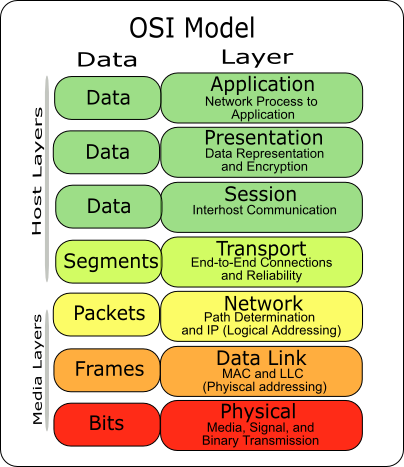
\includegraphics[width=\textwidth]{assets/osi/layers.png}
    \caption{The OSI Model Layers}
    \label{fig:osi_layers_intro}
\end{minipage}

\begin{table}[h]
    \centering
    \begin{tabular}{|c|c|c|}
        \hline
        \textbf{Layer} & \textbf{Function} & \textbf{Example Protocols} \\
        \hline
        Application & User interface and application services & HTTP, FTP, SMTP \\
        Presentation & Data translation and encryption & SSL/TLS, JPEG, MPEG \\
        Session & Establishes, manages, and terminates sessions & NetBIOS, RPC \\
        Transport & Reliable data transfer and flow control & TCP, UDP \\
        Network & Routing and addressing of data packets & IP, ICMP \\
        Data Link & Node-to-node data transfer and error detection & Ethernet, PPP \\
        Physical & Transmission of raw bit streams over physical medium & USB, Bluetooth \\
        \hline
    \end{tabular}
    \caption{The Seven Layers of the OSI Model}
    \label{tab:osi_layers}
\end{table}

We will cover these layers by example in the next chapters, drilling down into layer-specific protocols and their intersections.
